\section{Path Visibility Faults}\label{sec:visibility}

Recall that {\em path visibility} specifies that every router that has a
usable path to a destination learns at least one valid route to that
destination (Definition~\ref{defn:pv}). It is an important property
because it ensures that, if the network remains connected at lower
layers, the routing protocol does not create any network partitions.
Table~\ref{tab:rcc_tests} shows many conditions that \rcc checks related
to path visibility; in this section, we focus on iBGP configuration
faults that can violate path visibility and explain how \rcc detects
these faults.

%Routers within an AS disseminate eBGP-learned routes to
%other routers in the AS using iBGP.  
%If two routers in the same AS have the same loopback address, visibility
%can be violated if one of those routers hears a route from the
%other, and discards it, thinking it advertised the route itself.
%The simplest approach is to propagate routes within the AS involves
%configuring iBGP 
%sessions between every pair of BGP-speaking routers within the AS, (a
%``full-mesh'' topology), where each router selects a best route from
%among its available choices and, if that route was learned via eBGP,
%readvertises that route over its iBGP sessions.  

Ensuring path visibility in a ``full mesh'' iBGP topology (as described
in Section~\ref{sec:dissemination}) is reasonably
straightforward; \rcc checks that every router in the AS has an iBGP
session with every other eBGP-speaking router.  If this condition is
satisfied, every router in the AS will learn all eBGP-learned routes.

%Because a ``full mesh'' iBGP topology scales poorly, operators often
%employ {\em route reflection}~\cite{rfc2796}.  A subset of the
%routers are configured as {\em route reflectors}, with the configuration
%specifying a set of other routers as {\em route reflector clients}.
%Each route reflector readvertises its best route according to the
%following rules: (1)~if the best route was learned from an iBGP peer,
%the route is readvertised to all of its route reflector clients; (2)~if
%it was 
%learned from a client or via an eBGP session, the route is readvertised
%on all iBGP sessions.  
%If a route reflector client has
%multiple route reflectors, those reflectors must share all of their
%clients and belong to a single ``cluster''.

A route reflector may itself be a client of another route reflector.
Any router may also have iBGP sessions with other routers.
Recall from Section~\ref{sec:visibility_def} that we use the set of
reflector-client relationships between routers in an AS to define a 
graph $\I$, where each router is a node and each
session is either a directed or undirected edge: a client-reflector
session is a directed edge from 
reflector to client, and other iBGP sessions are undirected edges.  An
edge exists if and only if (1)~the configuration of each router endpoint
specifies the loopback address of the other endpoint\footnote{If a
router establishes an iBGP session with a router's {\em loopback} address,
then the iBGP session will remain active as long as that router is
reachable via {\em any} IGP path between the two routers.  If a router
establishes an iBGP session with an interface address of another router,
however, the iBGP session will go down if that interface fails, even if
an IGP path exists between those routers.} and (2)~both routers agree
on session options (\eg, MD5 authentication parameters).  $\I$
should also not have partitions at lower layers.  We say that $\I$ is
{\em acyclic} if $\I$ has no sequence of directed and undirected edges
that form a cycle.  

\begin{figure}[t]
\begin{center}
\begin{psfrags}
\psfrag{r1}{{\Large Route $r_1$ to $d$}}
\psfrag{r2}{{\Large Route $r_2$ to $d$}}
\psfrag{RR1}{{\LARGE $RR_1$}}
\psfrag{RR2}{{\LARGE $RR_2$}}
\psfrag{W}{{\LARGE $W$}}
\psfrag{X}{{\LARGE $X$}}
\psfrag{Y}{{\LARGE $Y$}}
%\centering
\begin{pspicture}(8,3.5)
%    \showgrid
    \psset{nodesep=2pt, arrows=->}

    \cnodeput(2.875,3.05){W}{$W$}
    \cnodeput(6,2.1){Y}{$Y$}
    \cnodeput(2,2.1){c1}{\hspace{0.12in}}
    \cnodeput(3.75,2.1){c2}{$X$}%\hspace{0.12in}}
    \cnodeput(6.875,1.15){c3}{$Z$}

    \ncline{c1}{W}
    \ncline{c2}{W}
    \ncline{c3}{Y}

    \psset{nodesep=2pt, arrows=-}
    \ncline{c2}{Y}


    \rput(2.875,4){\rnode{r1}{{\small route $r_1$ to $d$}}}
    \rput(3.75,0.25){\rnode{r2}{{\small route $r_2$ to $d$}}}

    \psset{nodesep=1pt, linestyle=dashed, arrows=<-}
    \ncline{W}{r1}
    \ncline{c2}{r2}%\rput(1.25,0.5){\rnode{w2}{$w_2$}}

    \rput(4.55,3.25){\rnode{rrc}{{\small Route Reflector (RR)}}}
    \rput(4.15,2.55){\rnode{rrc}{{\small Client}}}

    \rput(6.5,2.35){\rnode{rrc}{{\small RR}}}
    \rput(7.23,1.6){\rnode{rrc}{{\small Client}}}


    \psframe[fillcolor=white,linestyle=dashed, framearc=0.3](1.25,0.75)(7.75, 3.5)


\end{pspicture}

\resizebox{0.55\linewidth}{!}{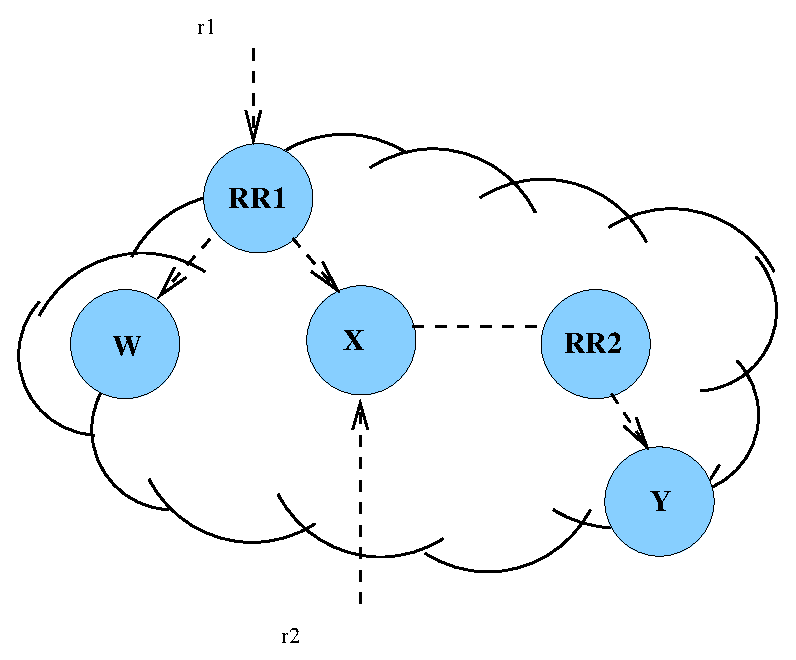
\includegraphics{rcc/figures/rr_example_fig2.eps}}
\end{psfrags}
\end{center}
\caption[An iBGP route reflector topology that violates path visibility.]{
In this iBGP configuration, route
$r_2$ will be distributed to all the routers in the AS, but
$r_1$ will not.  $RR_2$ and $Y$ will not learn of $r_1$, leading to a
network partition that won't be resolved unless another route to
the destination appears from elsewhere in the AS.}
\label{f:ibgp_vis_violation}
\end{figure}

%% \begin{figure}
%% \centering
\begin{pspicture}(8,3.5)
%    \showgrid
    \psset{nodesep=2pt, arrows=<->}

    \cnodeput(2,2.75){WC1}{$WC_1$}
    \cnodeput(1,1.6){WC2}{$WC_2$}
    \cnodeput(3,1.35){WC3}{$WC_3$}
    \cnodeput(6.25,2.75){EC1}{$EC_1$}


    \ncline{WC1}{WC2}
    \ncline{WC2}{WC3}
    \ncline{WC3}{WC1}

    \ncline{WC1}{EC1}
    \ncline{WC2}{EC1}
    \ncline{WC3}{EC1}

    \rput(1,0){\rnode{pw2}{}}
    \rput(3,0){\rnode{pw3}{}}
    \rput(6.25,0){\rnode{pe1}{}}


    \psset{nodesep=2pt, linestyle=dotted, arrows=<->}
    \ncline{WC2}{pw2}\rput(1.25,0.5){\rnode{w2}{$w_2$}}
    \ncline{WC3}{pw3}\rput(3.25,0.5){\rnode{w3}{$w_3$}}
    \ncline{EC1}{pe1}\rput(6.5,0.5){\rnode{e1}{$e_1$}}



    \psset{nodesep=0pt, arrows=-}

    \psframe[fillcolor=white,linestyle=dashed, framearc=0.3](0.25,0.75)(7.5, 3.5)


\end{pspicture}

%% \caption{BGP connectivity diagram for an AS with three routers on the
%%   west coast and one on the east coast.  Solid lines denote iBGP
%%   sessions, and dotted lines denote eBGP sessions.}
%% \label{fig:visibility_example}
%% \end{figure}

Even a connected directed acyclic graph of iBGP sessions can violate
path visibility.  For example, in Figure~\ref{f:ibgp_vis_violation},
routers $RR_2$ and $Y$ do not learn route $r_1$ to destination $d$ (learned
via eBGP by router $RR_1$), because $X$ will not readvertise routes learned
from its iBGP session with $RR_1$ to other iBGP sessions.  We call this
path visibility fault an {\em iBGP signaling partition}: a
path exists, but neither $RR_2$ nor $Y$ has a route for it.  Note that
simply adding a regular iBGP session between routers $RR_1$ and $RR_2$ would
solve the problem.

%This potentially active fault can
%prevent routers from learning any route to a destination, even
%though a path exists.  
In addition to causing network partitions, iBGP signaling partitions may
result in suboptimal routing.
For example, in Figure~\ref{f:ibgp_vis_violation}, even if $RR_2$ or $Y$
learned a route to $d$ via eBGP, that route might be worse than
the route learned at $RR_1$.  In this case, $RR_2$ and $Y$ would ultimately
select a suboptimal route to the destination, an event that an operator
would likely fail to notice.


%
%% Visibility violations have the potential for hard-to-detect network
%% partitions (mainly because the location of the problem could be far
%% from the place the misconfiguration has happened).  There are other
%% problems caused by lack of visibility too, as shown in
%% Figure~\ref{fig:visibility_example}.  Assume that $w_2$, $w_3$, and
%% $e_1$ are eBGP sessions to the same neighboring AS that advertises a
%% route to destination $d$.  If router $EC_1$ were misconfigured such
%% that it was not readvertising its routes to the $WC$ routers, then
%% none of the $WC$ routers would be able to reach $d$, even though a
%% valid path to $d$ exists via $EC_1$.  Moreover, if the AS in the
%% figure has routers separated by long-haul links (\eg the ``WC''
%% routers were on the West Coast of the US and the ``EC'' routers were
%% on the East Coast), and the route to $d$ were not advertised by either
%% $WC_2$ or $WC_3$, then these routers would send packets to $d$ via
%% $EC$ instead of sending packets via the nearest available exit point.
%% In this example, if the $WC_1\leftrightarrow WC_2$ and
%% $WC_1\leftrightarrow WC_3$ sessions were non-existent or had failed,
%% then $WC_1$ would choose the sub-optimal route to $d$ via $e_1$.
%

\rcc detects iBGP signaling partitions.
It determines if there is {\em any}
combination of eBGP-learned routes such that at least one router in the
AS will not learn at least one route to the destination, by performing a
check based on the following result, which we proved in
Section~\ref{sec:visibility_def}. 

\vskip 0.1in
%\begin{theorem}\label{thm:vis}

\noindent {\bf Theorem~\ref{thm:vis}.} 
{\em Suppose that the graph defined by an AS's iBGP relationships, $\I$, is
acyclic.  Then, $\I$ does not have a signaling partition if, and only
if, the eBGP-speaking routers that are not route reflector clients form
a clique. }
%\end{theorem}
\vskip 0.1in

%% \begin{proof}
%% Call the set of routers that are not reflector clients the
%% ``top layer'' of $G$.  If the top layer is not a full mesh,
%% then there are two routers $X$ and $Y$ with no iBGP session between
%% them, such that no route learned using eBGP at $X$ will ever be
%% disseminated to $Y$, since no router readvertises an
%% iBGP-learned route.

%% Conversely, if the top layer is a full mesh, observe that {\em if} a
%% route reflector 
%% has a route to the destination, then all its clients
%% have a route as well.  Thus, if every router in the
%% top layer has a route, all routers in the AS will have a route.  If any
%% router in the top layer learns a route through eBGP, then all the
%% top layer routers will hear of the route (because the top layer is a
%% full mesh).  Alternatively, if no router at the top layer hears an
%% eBGP-learned route, but some other router in the AS does, then that
%% route propagates up a chain of route reflectors (each client sends it to
%% its reflector, and the reflector sends it on all its iBGP sessions) to
%% the top layer, from there to all the other top layer routers, and from
%% there to the other routers in the AS.
%% \end{proof}


\rcc checks this condition by constructing the iBGP signaling
graph $\I$ from the {\tf sessions} table (Table~\ref{tab:if}). It assumes
that the IGP graph is connected, then determines whether $\I$ is
connected and acyclic and whether the routers at the top layer of $\I$ form
a clique.

